\documentclass[10pt,sigconf]{acmart}
\synctex=1
\graphicspath{{figures/}{doc/paper/}}
\usepackage[l2tabu,orthodox]{nag}
\usepackage[utf8x]{inputenc}
\usepackage[british]{babel}
\usepackage{microtype}
\usepackage[caption=false]{subfig}
\usepackage{graphicx}
\usepackage{url}
\usepackage{color}

\frenchspacing
\uchyph=0

\newcommand{\todo}[1]{\textbf{\textcolor{red}{To do: #1}}}
\newcommand{\idea}[1]{{\textcolor{blue}{#1}}}

%==================================================================================================
\begin{document}
\title{Does TCP New Congestion Window Validation Improve HTTP Adaptive Streaming Performance?}

\author{Mihail Yanev}
    \orcid{0000-0002-9814-1017}
    \affiliation{
      \institution{University of Glasgow}
      \streetaddress{School of Computing Science}
      \city{Glasgow}
      \postcode{G12 8QQ}
      \country{UK}
    }
    \email{m.yanev.1@research.gla.ac.uk}

  \author{Stephen McQuistin}
    \orcid{0000-0002-0616-2532}
    \affiliation{
    \institution{University of Glasgow}
    \streetaddress{School of Computing Science}
    \city{Glasgow}
    \postcode{G12 8QQ}
    \country{UK}
    }
    \email{sm@smcquistin.uk}

\author{Colin Perkins}
  \orcid{0000-0002-3404-8964}
  \affiliation{
    \institution{University of Glasgow}
    \streetaddress{School of Computing Science}
    \city{Glasgow}
    \postcode{G12 8QQ}
    \country{UK}
  }
  \email{csp@csperkins.org}

\copyrightyear{2022}
\acmYear{2022}
\setcopyright{acmlicensed}
\acmConference[NOSSDAV'22]{The 32nd edition of
  the Workshop on Network and Operating System Support for Digital Audio and
  Video}{June 17, 2022}{Athlone, Ireland}
\acmBooktitle{The 32nd edition of the Workshop on Network and Operating
  System Support for Digital Audio and Video (NOSSDAV'22), June 17, 2022,
  Athlone, Ireland}
\acmPrice{15.00}
\acmDOI{10.1145/3534088.3534347}
\acmISBN{978-1-4503-9383-6/22/06}

\begin{CCSXML}
<ccs2012>
  <concept>
       <concept_id>10003033.10003039.10003048</concept_id>
       <concept_desc>Networks~Transport protocols</concept_desc>
       <concept_significance>300</concept_significance>
  </concept>
  <concept>
    <concept_id>10003033.10003039.10003051</concept_id>
    <concept_desc>Networks~Application layer protocols</concept_desc>
    <concept_significance>300</concept_significance>
  </concept>
  <concept>
       <concept_id>10003033.10003079.10003081</concept_id>
       <concept_desc>Networks~Network simulations</concept_desc>
       <concept_significance>100</concept_significance>
  </concept>
  <concept>
    <concept_id>10003033.10003068.10003073.10003075</concept_id>
    <concept_desc>Networks~Network control algorithms</concept_desc>
    <concept_significance>500</concept_significance>
  </concept>
 </ccs2012>
\end{CCSXML}

\ccsdesc[300]{Networks~Transport protocols}
\ccsdesc[300]{Networks~Application layer protocols}
\ccsdesc[100]{Networks~Network simulations}
\ccsdesc[500]{Networks~Network control algorithms}

\keywords{TCP, MPEG DASH, Congestion Window Validation}

%==================================================================================================
\begin{abstract}

  
  % Four sentences:
  %  - State the problem
  %  - Say why it's an interesting problem
  %  - Say what your solution achieves
  %  - Say what follows from your solution

When using HTTP adaptive streaming, video traffic exhibits on-off behaviour with frequent idle periods that can interact poorly with TCP congestion control algorithms. New congestion window validation (New CWV) modifies TCP to allow senders to recover their sending rate more quickly after certain idle periods. While previous work has shown that New CWV can improve \emph{transport} performance for streaming video, it has not been shown if this translates to improved \emph{application} performance in terms of playback stability. In this paper, we show that New CWV can reduce video re-buffering events by up to 4\%, and limit representation switches by 12\%, without any changes to existing rate adaptation algorithms.

\end{abstract}
\maketitle
%==================================================================================================
\section{Introduction}
\label{sec:introduction}

Video streaming over HTTP is commonplace, and comprises the majority of Internet traffic~\cite{Sandvine-2019-global-internet-report}. The performance of such HTTP adaptive streaming video is generally very good, and gives a high-quality user experience.
  
There are, however, some scenarios where HTTP adaptive streaming can perform comparatively poorly \cite{Spiteri-2016-BOLA,Kua-2017-a-survey-rate-adaptation-dash}. In particular, interactions between the on-off traffic patterns generated by adaptive streaming applications and TCP congestion control can reduce the performance of throughput-based video rate adaptation schemes~\cite{Akhshabi-2012-http-adaptive-players-compete,Stohr-2017-where-are-the-sweet-spots-maci}. In some cases, this is due to the TCP congestion window validation (CWV) \cite{rfc2861-2000-padhye-congestion-window-validation} algorithm that, while preventing TCP clients from sending using stale knowledge of the network, has been shown to negatively impact throughput of rate-limited applications~\cite{Nazir-2014-performance-evaluation-congestion-window-validation-dash-newcwv}, including adaptive streaming. New congestion window validation (New CWV)~\cite{rfc7661-2015-fairhurst-new-cwnd-validation} has been proposed to address this. Prior work~\cite{Nazir-2014-performance-evaluation-congestion-window-validation-dash-newcwv} has demonstrated that New CWV has the desired \emph{transport} layer impact, but it remains to show that this translates to improved \emph{application} quality of experience (QoE). This is not guaranteed due to the complexity of, and interactions between, transport and application. For example, large discrepancies between video bandwidth requirements and the available link capacity, or the requirement for stable, long-lived connections can influence rate adaptation \cite{Spiteri-2019-from-theory-to-practice-sabre}.

In this paper, we investigate whether enabling New CWV improves video playback stability and, more generally, video QoE for HTTP adaptive streaming over TCP. We compare video performance using TCP New Reno with the CWV and New CWV algorithms. We collect standard video performance metrics, including bit-rate oscillation, and stall time, to measure stability and QoE. Further, to quantify the impact of New CWV with respect to the inferred network state at the client, we also record the immediate and smoothened client's link capacity estimations for each delivered chunk.

We make the following contributions: (i) we implement New CWV for Linux kernel 5.4; (ii) we evaluate the application layer impact of New CWV; and (iii) we demonstrate that New CWV improves video stability, with a 12\% reduction in bit rate switches, and a 4\% reduction in rebuffering time.


To the best of our knowledge, we are the first to study the application
layer impact of enabling New CWV. 
Nazir et al. \cite{Nazir-2014-performance-evaluation-congestion-window-validation-dash-newcwv}
demonstrated the effect of New CWV on the transport layer, and there has been a large amount of work that has proposed new application layer rate adaptation algorithms \cite{Mok-2012-qdash,Huang-2015-A-buffer-based-approach-to-rate-adaptation-bba, Yin-2015-a-control-theoritic-approach}. In contrast, we only change the transport, leaving the application as is, to study the transport impact on the application. Improving performance via transport layer modifications could allow for simpler rate adaptation algorithms at the application layer.


We structure the remainder of this paper as follows. In Section~\ref{sec:background}, we introduce TCP congestion window validation, including its limitations with respect to HTTP adaptive video flows, before describing New CWV. Section~\ref{sec:evaluation} describes our experimental setup, and the transport and application layer impact of enabling New CWV. Section~\ref{sec:related} describes related work, and Section~\ref{sec:conclusion} concludes.

%==================================================================================================
\section{Congestion Window Validation}
\label{sec:background}

\begin{figure}
  \centering
    \subfloat[CWV]{
      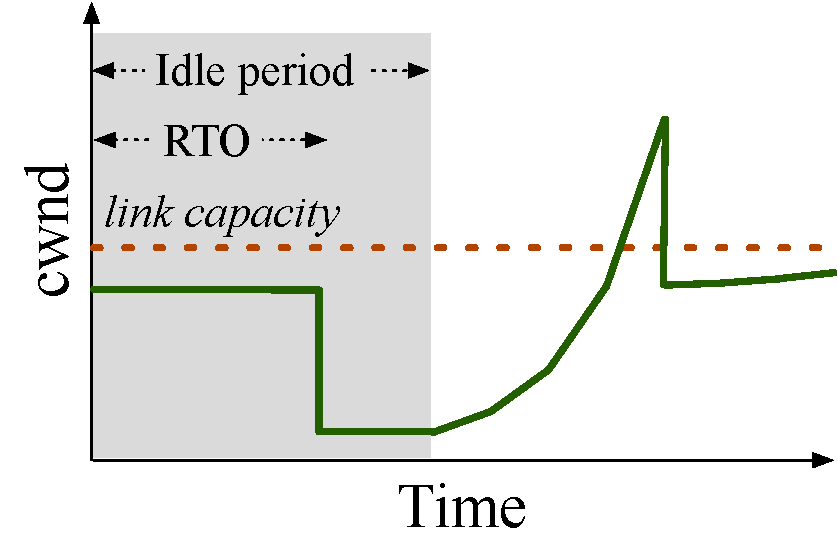
\includegraphics[width=.23\textwidth]{figures/cwv.pdf}
      \Description{Illustration of cwnd growth over time, with Congestion Window Validation enabled.}
      \label{fig:cwv}
    }
    \subfloat[New CWV]{
      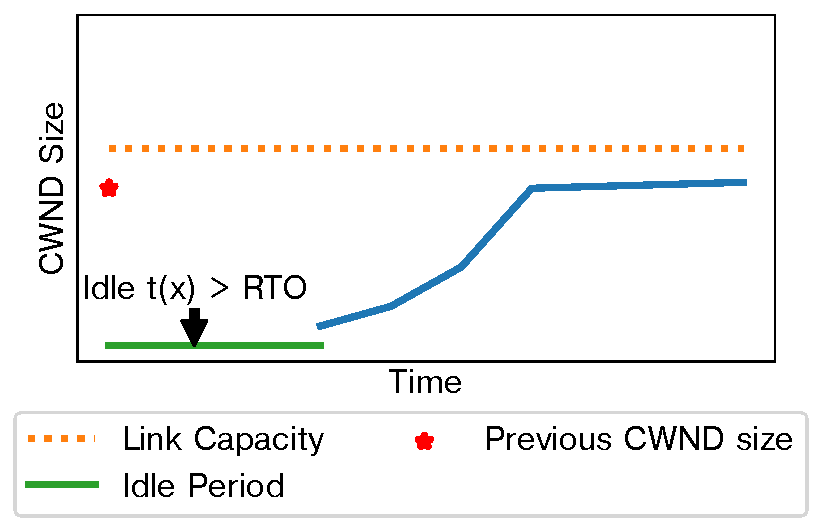
\includegraphics[width=.23\textwidth,]{figures/new_cwv.pdf}
      \Description{Illustration of cwnd growth over time, with New Congestion Window Validation enabled.}
      \label{fig:newcwv}
    }
    \caption{\emph{cwnd} growth following an idle period}
    \label{fig:cwnd-growth-after-idle}
\end{figure}

In HTTP adaptive streaming, a server provides pre-encoded video chunks in different representations, each encoded at multiple bit rates. The client use a rate adaptation algorithm to determine the best representation to request at any given time. The goal of the client is to maximise QoE within the network's capacity. This can be a challenge since different, often contradictory, QoE heuristics need be considered \cite{Seufert-2015-A-Survey-on-QoE-Dash}. 

Throughput-based rate adaptation algorithms require a stable and accurate estimate of TCP throughput. However, interactions between the on-off traffic pattern of streaming video and TCP congestion control can cause significant fluctuations in TCP behaviour, impacting performance.


In particular, during idle periods in between transmission of video chunks, the TCP congestion controller's knowledge of the network capacity becomes stale. To avoid sending with a possibly unrepresentative congestion window, once the link has been idle for a period longer than the retransmission timeout, $T_{rto}$, the congestion window validation~\cite{rfc2861-2000-padhye-congestion-window-validation} (CWV) algorithm resets the TCP congestion window (\emph{cwnd}) to its initial value and forces the connection to re-enter slow-start. Figure~\ref{fig:cwv} illustrates this behaviour. CWV has become standard practice~\cite{rfc5681-congeston-control}, and is enabled by default in the latest stable Linux kernel (5.4). This slow start after idle, however, causes bursts of packet loss when the \emph{cwnd} overshoots the link capacity at the end of the slow start (Figure~\ref{fig:transmission-after-idle-reno}). This can to interact poorly with HTTP adaptive streaming and other application-limited transmissions~\cite{Esteban-2012-Interactions-HTTP-TCP}.

To address this, new congestion window validation~\cite{rfc7661-2015-fairhurst-new-cwnd-validation} was proposed. During slow start after idle, rather than relying on packet loss to re-discover its appropriate \emph{cwnd} value, New CWV preserves the \emph{cwnd} before the idle period and later uses it as the slow start threshold (\emph{ssthresh}). That is, it exits the slow-start phase before loss occurs, assuming no change in available bandwidth. Figure~\ref{fig:newcwv} shows the growth of \emph{cwnd} following an idle period under New CWV.

\begin{figure}[t!]
  \centering
  \subfloat[New CWV]{
    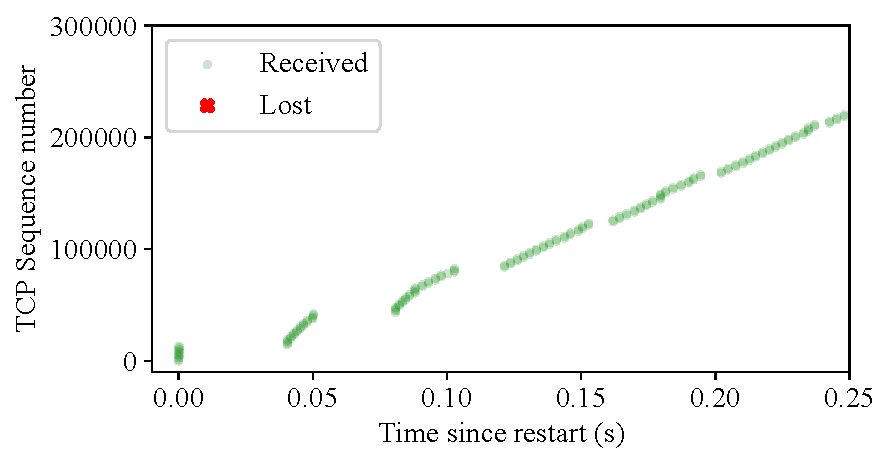
\includegraphics[width=.45\textwidth, keepaspectratio]{figures/lost_packets_newcwv.pdf}
    \Description{Scatter plot showing the impact of New Congestion Window Validation on tail packet losses across several flights of packets. New Congestion Window Validation allows packet loss to be avoided.}
    \label{fig:transmission-after-idle-newcwv}
  }
  \\
  \subfloat[CWV]{
    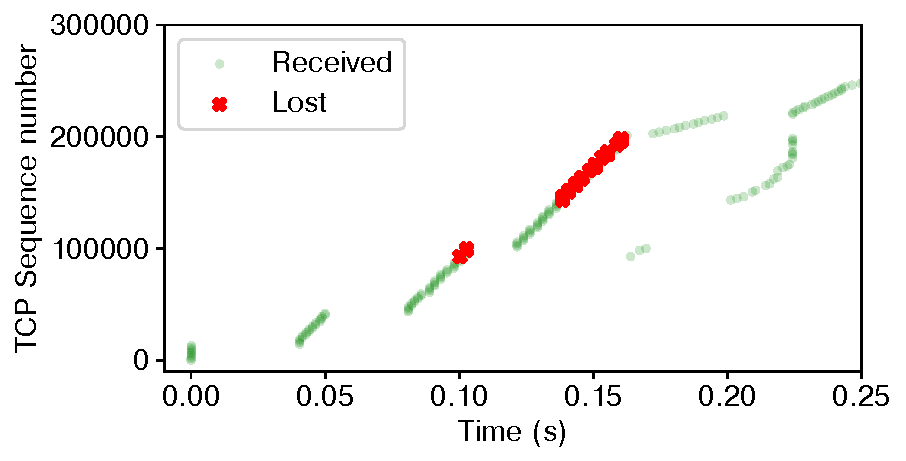
\includegraphics[width=.45\textwidth, keepaspectratio]{figures/lost_packets_vreno.pdf}
    \Description{Scatter plot showing the impact of Congestion Window Validation on tail packet losses across several flights of packets. Congestion Window Validation, in relying on packet loss to exit slow start, causes tail loss for several flights of packets.}
    \label{fig:transmission-after-idle-reno}
  }
  \caption{Resumption after an idle period}
  \label{fig:transmission-after-idle}
\end{figure}

We implemented New CWV in Linux\footnote{A snapshot of our implementation, as used in this paper, is available at \url{http://dx.doi.org/10.5525/gla.researchdata.1278}, while the main repository for the work is at \url{https://github.com/glasgow-ipl/newcwv-nossdav2022}.}. We used \cite{secchi-2016-newcwv} as a base, which provides an implementation for Linux 3.18, and ported the changes to Linux 5.4. Our implementation altered two files, adding 143 and removing 49 lines of code.

We use this implementation to better illustrate the impact of New CWV on flows restarting after an idle period, as shown in Figure \ref{fig:transmission-after-idle}.
The New CWV connection (Figure \ref{fig:transmission-after-idle-newcwv}) uses the previously set \emph{ssthresh} value and leaves slow-start early, avoiding packet loss, after reaching the \emph{ssthresh} in the third flight of packets after restarting. 
In contrast, if the same connection used CWV, the senders would not have preserved the \emph{ssthresh} value and would rely on loss to exit slow-start, as seen at the end of the third and fourth flights of packets in Figure \ref{fig:transmission-after-idle-reno}. In this example, the connection using CWV enters congestion avoidance \textasciitilde160ms after transmission restarts, while that using New CWV is able to enter congestion avoidance \textasciitilde50ms earlier and avoid packet loss.
Overall, New CWV results in fewer lost packets, and returns to its previous sending rate without overshoot after loss, giving more predictable transmission.

New CWV has been shown to improve \emph{transport} layer performance of rate-limited applications when compared with CWV~\cite{Nazir-2014-performance-evaluation-congestion-window-validation-dash-newcwv}, and the results we have presented here validate that, although it remains to show how this translates into \emph{application} layer performance \cite{Spiteri-2016-BOLA}. 

%==================================================================================================
\section{Evaluating New CWV for Video}
\label{sec:evaluation}

\begin{figure}
  \centering
  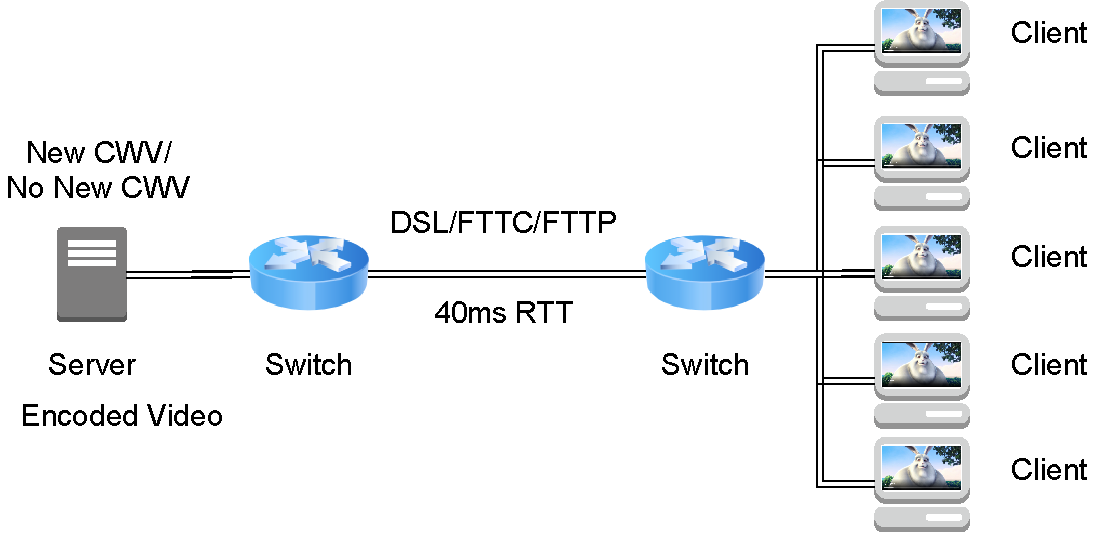
\includegraphics[width=.45\textwidth]{figures/setup.pdf}
  \Description{Illustration of the experimental setup. The server, running Congestion Window Validation or New Congestion Window Validation, serves encoded video over an emulated link to up to 5 clients.}
  \caption{Experimental Setup}
  \label{fig:experimental-setup}
\end{figure}

In this section, we first validate the results of Nazir et al.~\cite{Nazir-2014-performance-evaluation-congestion-window-validation-dash-newcwv}, before testing whether New CWV will enable \emph{applications} to obtain more consistent throughput estimates, and, in turn, improve the stability of rate adaptation algorithms.
We first describe our experimental setup (\S\ref{sec:experimental-setup}). Second, we investigate the transport layer impact to check if New CWV connections obtain more consistent throughput estimates (\S\ref{sec:transport-impact}). Then, we investigate the application impact, specifically the difference on video QoE due to New CWV (\S\ref{sec:QoE-impact}). Finally, we summarise our findings (\S\ref{sec:summary}).

%--------------------------------------------------------------------------------------------------
\subsection{Experimental Setup}
\label{sec:experimental-setup}

% Overview
Our evaluation consists of a network emulated in Mininet, running on Ubuntu 20.04, as shown in Figure~\ref{fig:experimental-setup}. Both the server and clients use TCP New Reno and run Linux Kernel 5.4.0 modified to include New CWV and RFC 3339~\cite{rfc3339-precise-timestamps} compliant timestamps to enable high precision event tracking. 

% Server
The server uses \texttt{nginx} (v1.18) with HTTP/2, serving three representations of Big Buck Bunny\footnote{\url{https://download.blender.org/demo/movies/BBB/}}: 480p (0.44Mbps), 720p (2.64Mbps), and 1080p (4.82Mbps). Each is encoded in chunks of 3 seconds duration.
%  Client
Clients use Firefox (v91) with \texttt{dash.js}\footnote{\url{https://github.com/Dash-Industry-Forum/dash.js}} (v4.0.0). We
report results with both the \textsc{throughput} and \textsc{dynamic} \cite{Spiteri-2019-from-theory-to-practice-sabre} algorithms implemented in \texttt{dash.js}.

The network is configured with an RTT of 40ms, matching a typical RTT to a nearby CDN node. The routers' queues are sized to the bandwidth delay product. Three different bandwidth profiles are evaluated, representing ADSL2 (10Mbps), FTTC (50Mbps), and FTTP (145Mbps) links. We show the results for ADSL2 and FTTC links.
While FTTP links are common in some regions, ADSL2 and FTTC links are still widely used \cite{ofcom-2020-report,FCC-measuring-broadband-america,EC-measuring-broadband-europe,ACCC-measuring-broadband-australia}. As higher resolution video and other network-heavy operations such as virtual reality environments see more use we expect issues observed with ADSL2 and FTTC will translate to the higher capacity FTTP links.
We send only video traffic and assume a consistent RTT, broadly modelling a home environment with multiple people watching simultaneous video streams and little other traffic. Evaluating effects of cross traffic and video synchronisation is future work.

To evaluate the impact of congestion and competing flows, experiments were run with both \textsc{dynamic} and \textsc{throughput} algorithms and several (1, 2, 3, and 5) simultaneous clients. Finally, to reduce noise, we ran each combination of CWV or New CWV, adaptive algorithm, number of clients, and link type, 10 times before reporting the average results. The results presented includes data accumulated from 480 simulations (2 congestion control algorithms $\times$ 2 adaptive algorithms $\times$ 3 link types $\times$ 4 client variations $\times$ 10 repetitions). 
During each run we collect client bandwidth estimates. Additionally, to evaluate the video QoE impact we report the rebuffer ratio and bitrate switch frequency distribution.

%--------------------------------------------------------------------------------------------------
\subsection{Impact on Transport Performance} 
\label{sec:transport-impact}

New CWV alters TCP \emph{cwnd} sizing behaviour, allowing it to recover more quickly after idle periods, and, as shown in Section \ref{sec:background}, prevents packet loss when exiting slow start which should give more stable bandwidth estimates. 

To evaluate this, we collect instantaneous and smoothed bandwidth estimates from the clients. The instantaneous estimate is obtained by dividing the size of the chunk by the time taken to download it. The smoothed estimate is a function of the instantaneous estimate and other variables, f.e., historical measurement data and safety or ``dampening'' factors. The former is the throughput measurement as seen by the end-point, while the latter is the input value to the client's rate adaptation algorithm.

\begin{figure*}[t!]
  \centering
  \subfloat[ADSL2]{
    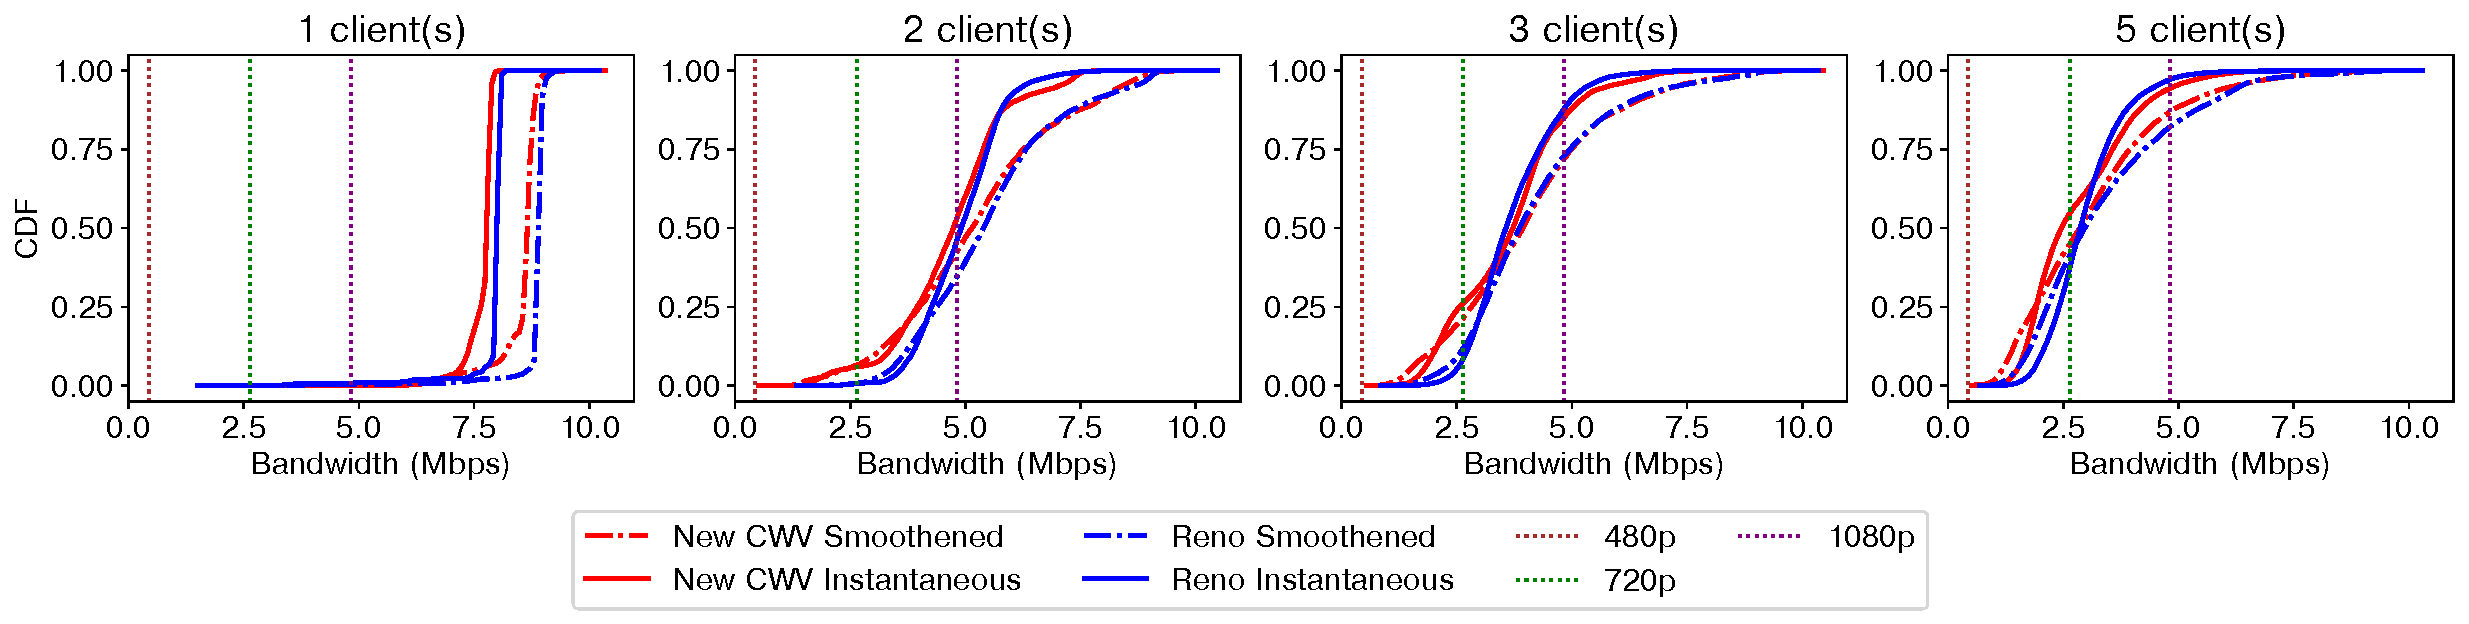
\includegraphics[width=\textwidth]{figures/Throughput_DSL.pdf}
    \Description{Cumulative Distribution Function plots showing the distribution of bandwidth estimates under the emulated DSL link, for 1, 2, 3, and 5 clients, comparing New Congestion Window Validation with Congestion Window Validation.}
    \label{fig:throughput-clients-DSL}
  }
  \\
  \subfloat[FTTC]{
    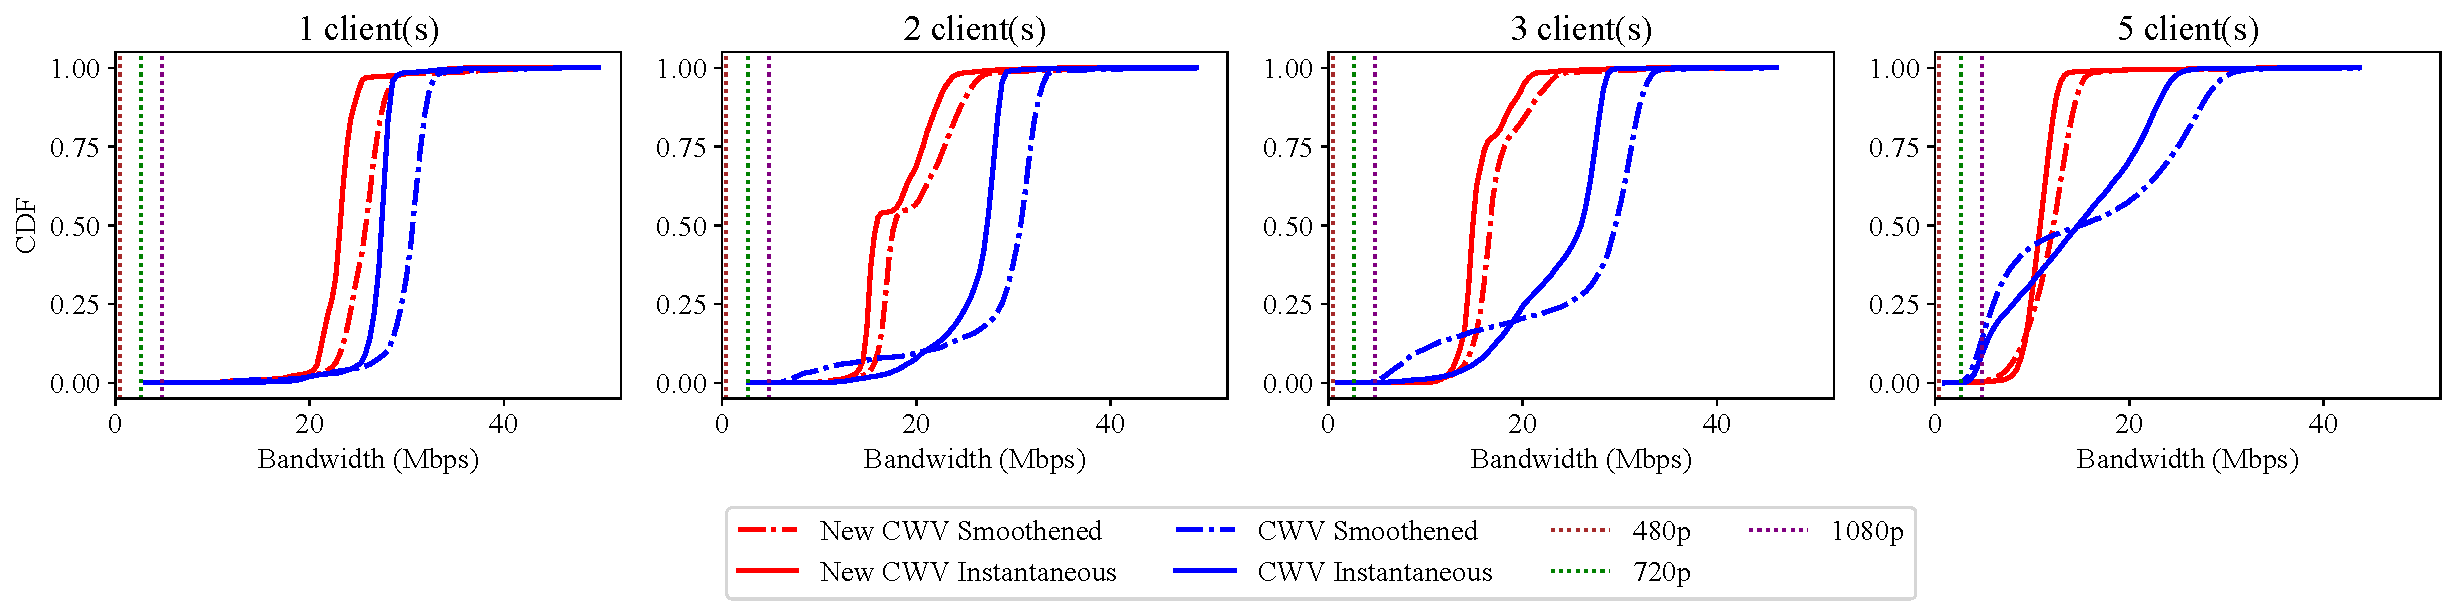
\includegraphics[width=\textwidth]{figures/Throughput_FTTC.pdf}
    \Description{Cumulative Distribution Function plots showing the distribution of bandwidth estimates under the emulated FTTC link, for 1, 2, 3, and 5 clients, comparing New Congestion Window Validation with Congestion Window Validation.}
    \label{fig:throughput-clients-FTTC}
  }
  \caption{Measured dash.js client bandwidth estimates}
  \label{fig:throughput-clients}
\end{figure*}

The cumulative distribution of instantaneous and smoothed throughput is shown in 
Figure~\ref{fig:throughput-clients}. 
%
The ADSL2 results, Fig.\ \ref{fig:throughput-clients-DSL}, show \todo{what?}
%
The FTTC results, Fig.\ \ref{fig:throughput-clients-FTTC}, show a consistently tighter distribution with New CWV than CWV, representing a more stable throughput estimate. The exception is when only one client is used, where the link capacity was much higher than the total video bandwidth that could be requested; preventing the client from obtaining an accurate estimation of the available capacity.
%
FTTP results are not shown, since in no case was the link capacity reached, and there were no significant difference in performance between CWV and New CWV.

\todo{Not clear what the following is trying to say}
We note that cross-traffic is likely in real deployments. We also note that even in this case New CWV's video stability was higher as shown in Section \ref{sec:QoE-impact}. For all other cases, since clients were able to leave slow-start earlier, having less oscillating \emph{cwnd} compared to that of clients using CWV and have expectedly shown a steeper CDF throughput function. 

In addition to being more consistent, 
Clients with New CWV enabled reported throughput estimates that were lower overall.
This is matches the results in Section \ref{sec:background}, showing flows using New CWV leaving slow start earlier.
Nazir et al.~\cite{Nazir-2014-performance-evaluation-congestion-window-validation-dash-newcwv} also saw this behaviour. This also supports our initial hypothesis that streaming clients measuring throughput will be able to obtain estimates that are more stable. 

\begin{figure}[t!]
  \centering
  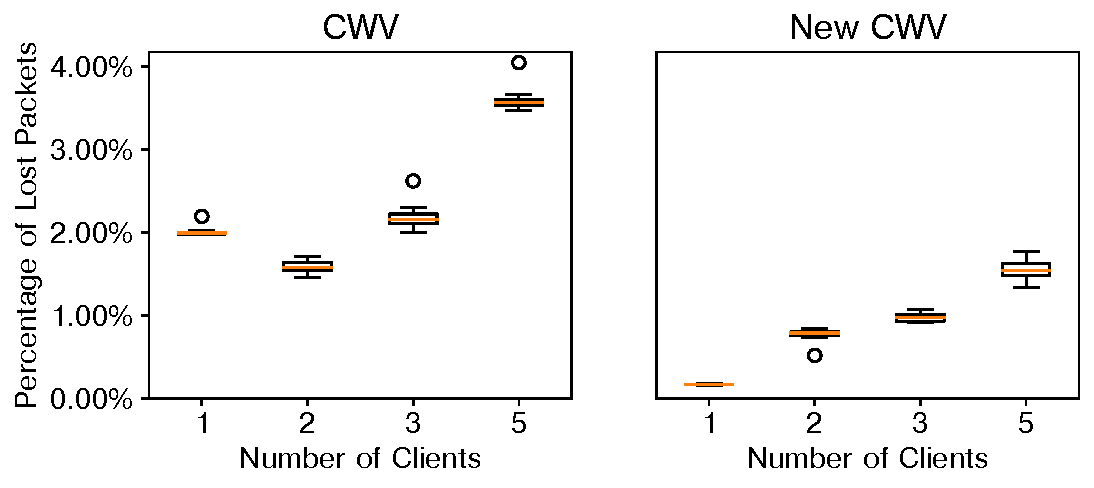
\includegraphics[width=.45\textwidth]{figures/lost_packets.pdf}
  \Description{Boxplots showing the percentage of packets loss under the emulated DSL link, for 1, 2, 3, and 5 clients, comparing New Congestion Window Validation with Congestion Window Validation.}
  \caption{Lost Packets DSL \todo{adaptation algo?}}
  \label{fig:lost-packets}
\end{figure}

We illustrate the impact of New CWV on packet loss in Figure~\ref{fig:lost-packets}. New CWV consistently achieves lower loss compared to CWV, with the former having packet loss rates that are less thsn half the latter. This confirms our hypothesis for loss, and matches Section \ref{sec:background}: New CWV exits slow-start earlier, does not overshoot its window, and therefore is able to avoid loss at the end of slow-start.

The loss values shown in Fig.\ \ref{fig:lost-packets} are reported for the \textsc{dynamic} rate adaptation algorithm. Results for the \textsc{throughput} algorithm show no significant differences.
\todo{Is this just true for loss, or for all the results in this section?}

%--------------------------------------------------------------------------------------------------
\subsection{Impact on Video QoE}
\label{sec:QoE-impact}

\begin{figure*}
  \centering
  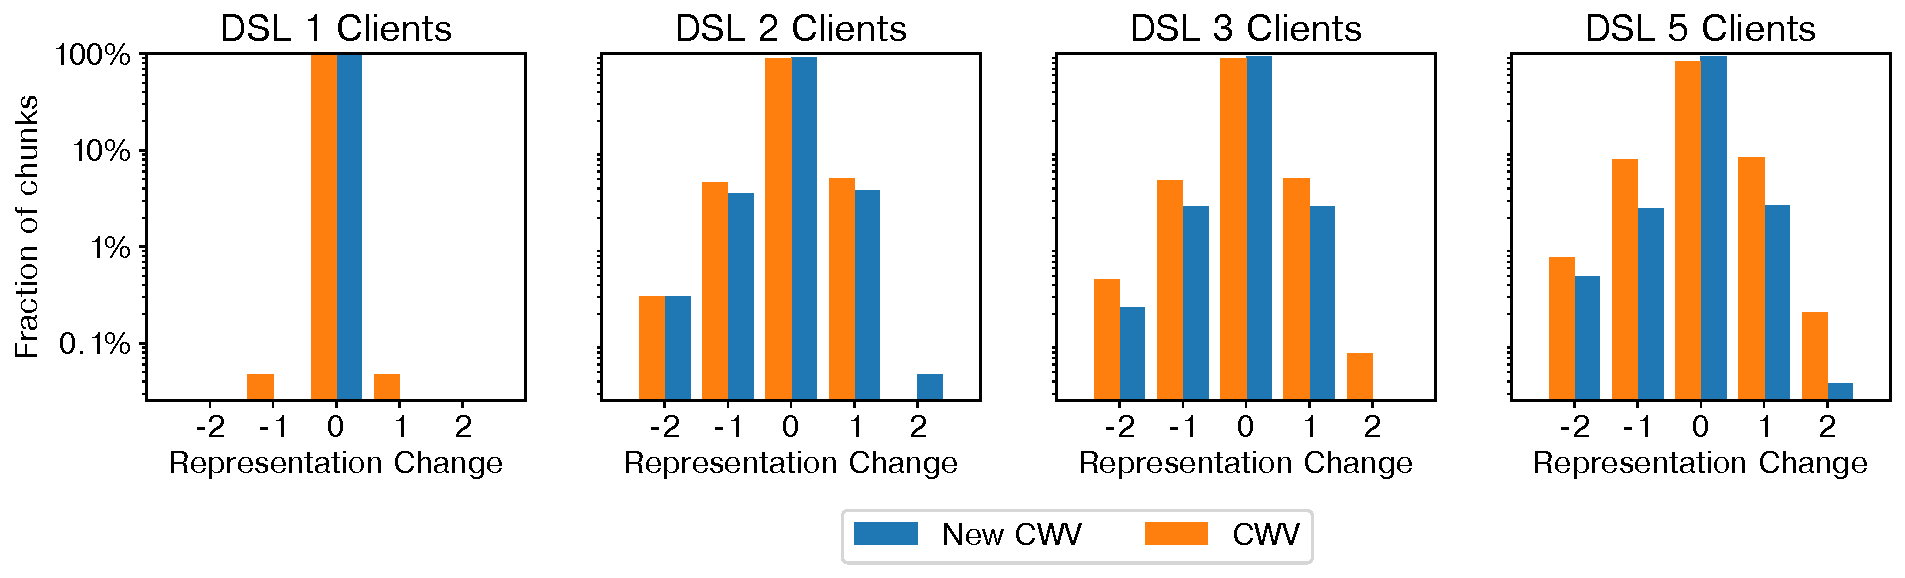
\includegraphics[width=\textwidth, keepaspectratio]{figures/bitrate_derivative_distribution.pdf}
  \Description{Bar plots showing the distribution of representation changes under the emulated DSL link, for 1, 2, 3, and 5 clients, comparing New Congestion Window Validation with Congestion Window Validation.}
  \caption{Absolute Bitrate Switches (\textsc{throughput})}
  \label{fig:bitrate-switches}
\end{figure*}

\begin{figure*}
  \centering
  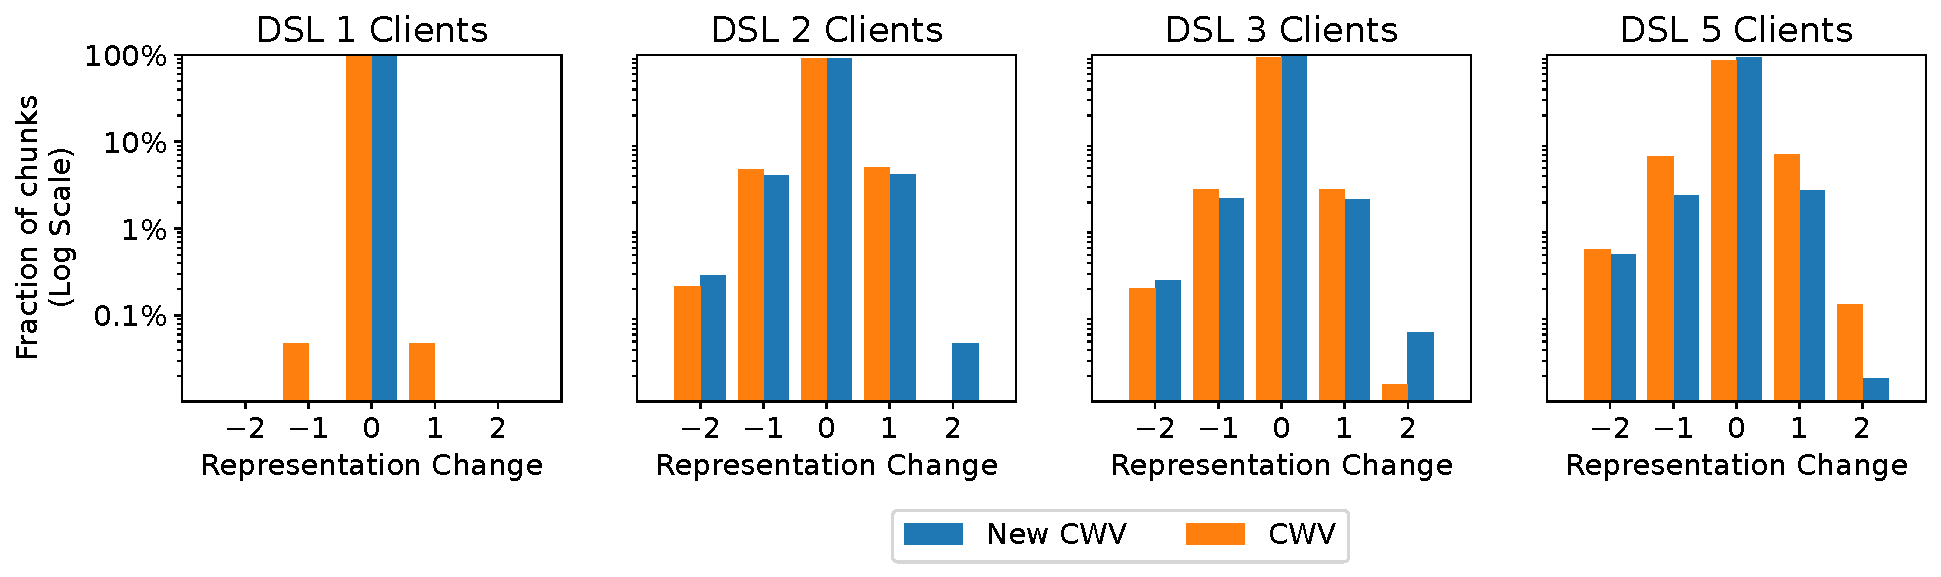
\includegraphics[width=\textwidth, keepaspectratio]{figures/bitrate_derivative_distribution_dynamic.pdf}
  \Description{Bar plots showing the distribution of representation changes under the emulated FTTC link, for 1, 2, 3, and 5 clients, comparing New Congestion Window Validation with Congestion Window Validation.}
  \caption{Absolute Bitrate Switches (\textsc{dynamic})}
  \label{fig:bitrate-switches-dynamic}
\end{figure*}


\begin{figure}
    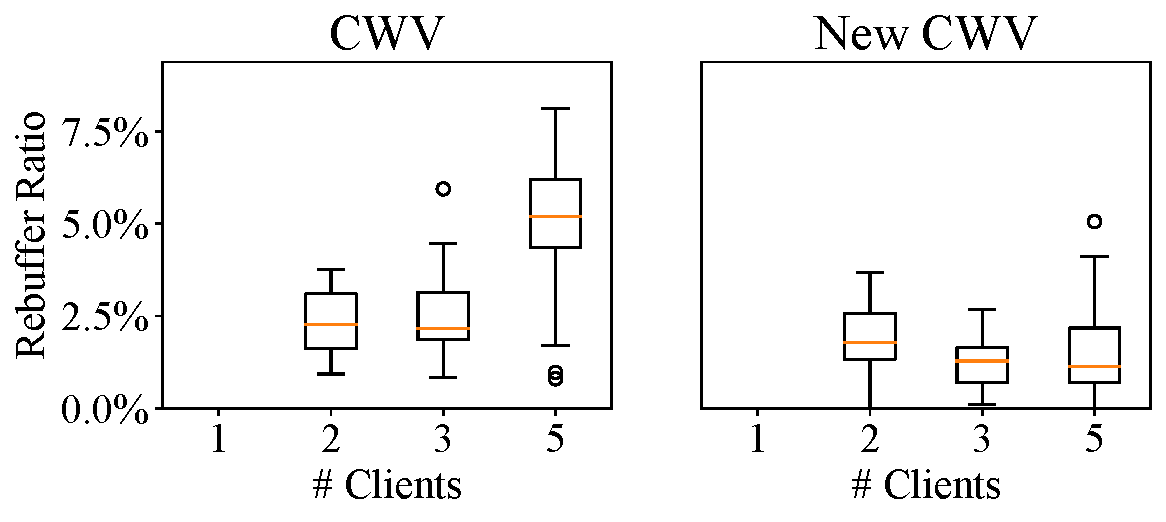
\includegraphics[width=.45\textwidth, keepaspectratio]{figures/Rebuffer_Ratio.pdf}
    \Description{Boxplots showing the rebuffer ratio under the emulated DSL link, with the throughput algorithm, for 1, 2, 3, and 5 clients, comparing New Congestion Window Validation with Congestion Window Validation.}
    \caption{Rebuffer Ratio (\textsc{throughput}) \todo{link type?}}
    \label{fig:rebuffer-ratio}
\end{figure}

\begin{figure}
    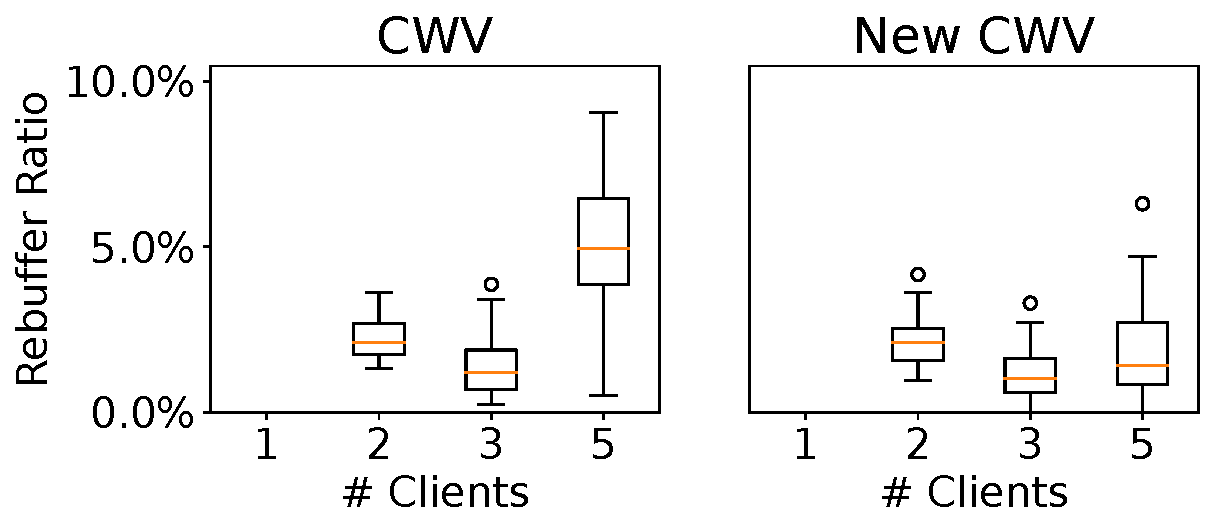
\includegraphics[width=.45\textwidth, keepaspectratio]{figures/Rebuffer_Ratio_dynamic.pdf}
    \Description{Boxplots showing the rebuffer ratio under the emulated DSL link, with the dynamic algorithm, for 1, 2, 3, and 5 clients, comparing New Congestion Window Validation with Congestion Window Validation.}
    \caption{Rebuffer Ratio (\textsc{dynamic}) \todo{link type?}}
    \label{fig:rebuffer-ratio-dynamic}
\end{figure}

To evaluate whether improved New CWV transport layer performance translates into improved application QoE, we explore impact on application-level metrics such as rebuffer ratio and bit rate switch frequency. 

In all cases, we report results for ADSL2 only. This link type, in combination with the video encodings used, best highlights scenarios where New CWV is beneficial. With FTTP links, all clients were able to stream at the highest quality without hitting the link limits. This was also the case for the FTTC links, with the exception of the 5 client scenario where we observed a similar pattern as that shown for ADSL2. Congestion control changes, such those we discuss, are ineffective when video flows are application limited and cannot cause congestion. Future higher-bandwidth applications, such as higher quality video, AR, or VR, will shift the congestion threshold upwards.

Figure \ref{fig:bitrate-switches} shows the bit rate switch distribution for the \textsc{throughput} algorithm; Figure \ref{fig:bitrate-switches-dynamic} shows \textsc{dynamic}.\footnote{The representation change (\emph{x-axis}) is the magnitude of the chunk-by-chunk bit rate switches. For example, if a chunk is requested at the same bit rate as the preceding chunk, the difference is zero. If the chunk is of the next higher encoding, compared to its predecessor, the difference is 1, and if it is of the next lower encoding the difference is -1, and so on.} 
In the extreme, with 5 clients, connections with CWV experience representation changes between 17.4\% of video chunks, compared to 5.7\% for connections with New CWV. Fewer clients congest the link less, and see correspondingly fewer shifts.

Comparing Figures~\ref{fig:bitrate-switches} and~\ref{fig:bitrate-switches-dynamic}, we see that when CWV is used, \textsc{dynamic} shows a significant reduction in representation changes compared to \textsc{throughput}. Connections using New CWV exhibit fewer representations shifts, irrespective of the rate adaptation algorithm, and are less affected by the choice of rate adaptation.


Figure \ref{fig:rebuffer-ratio} shows the fraction of the video playback where the connection has stalled when using the \textsc{throughput} algorithm. The value is shown in percentage relative to the whole media playtime. We see that New CWV experiences less rebuffering overall. The mean rebuffering values for the 5 client case are 5\% and 1.5\% for CWV and New CWV respectively, and correspondingly less for fewer clients. 
Figure \ref{fig:rebuffer-ratio-dynamic} shows results for \textsc{dynamic}, and again we see that the performance of the connections using CWV has improved, rebuffer-ratio is lower. Performance of New CWV connections does not differ significantly from what was already observed with \textsc{throughput}, and is still better than the performance with CWV even in cases where \textsc{dynamic} was used.

We do not present average bit rate results, due to space limitations, but these show little variation between CWV and New CWV. Differences that exist show slightly improved stability for New CWV, consistent with our other results.


Overall, New CWV achieves higher video stability when multiple clients are competing on a constrained link, with improved encoding stability and decreased rebuffering time. 
We observe that when New CWV is enabled, application metrics achieved for connections using either \textsc{dynamic} and \textsc{throughput} are very similar. A more complex rate adaptation algorithm, such as \textsc{dynamic}, has a significant impact on connections using CWV, but still gives lower QoE than the simpler adaptation algorithm used with New CWV.

%--------------------------------------------------------------------------------------------------
\subsection{Summary}
\label{sec:summary}

% Compared to \cite{Nazir-2014-performance-evaluation-congestion-window-validation-dash-newcwv} Figure~\ref{fig:throughput-clients} observed similar throughput distribution pattern. We observed lower loss for New CWV connections than they documented. We note that our environment tries to represent a more realistic case for video streaming as of the time of writing this paper. We have reconstructed their environment and used incremental RTT values starting from 40 (the value we used) going to 200 ms (the value they used) in incremental steps of 10 ms. We confirm that as the RTT increases New CWV connections experience higher loss and start to show closer results to when CWV is used. However, even with our incremental RTTs we have not managed to get higher but not as high loss rate as the one reported by the original authors. We attribute this difference to the fact that they used an older version of New Reno and their adaptive algorithm was very different to the current, dash.js, ones. 

The use of New CWV contributes to more consistent bandwidth estimates (Figure~\ref{fig:throughput-clients}) and leads to to fewer lost packets (Figure~\ref{fig:lost-packets}), fewer representation switches (Figures \ref{fig:bitrate-switches} \& \ref{fig:bitrate-switches-dynamic}), and lower rebuffering ratio (Figures \ref{fig:rebuffer-ratio} \& \ref{fig:rebuffer-ratio-dynamic}).
This is since the more consistent measurements better match the available network conditions, allowing clients using New CWV to better adapt to the constraints of the bottleneck link. 

The scenarios investigated by this work have used links that emulated a wired
residential Internet connection.  WiFi and cellular links, however, are known
to have very different properties that can affect TCP performance. Understanding
how use of TCP New CWV affects video performance on such links is outside the
scope of this current work.

Our experiments investigated the effects of New CWV on video delivered
using TCP New Reno. This was done to align with
\cite{Nazir-2014-performance-evaluation-congestion-window-validation-dash-newcwv},
and because a recent study \cite{Mishra-2019-the-great-internet-tcp-congestion-control-census}
found New Reno was still widely used for video delivery.
%
TCP Cubic grows its congestion window in slow start using the HyStart++
algorithm \cite{draft-ietf-tcpm-hystartplusplus}, and TCP BBRv2 tracks
bandwidth estimates during slow start, in both cases to avoid the overshoot
problems we discuss in Section \ref{sec:background} and improve stability.
These can potentially benefit from retaining state after idle periods in
the manner of New CWV; exploring this is for future work.

We consider similar scenarios to \cite{Nazir-2014-performance-evaluation-congestion-window-validation-dash-newcwv}, but our work was built to match scenarios that could be seen in 2022. Our findings broadly match theirs, consistent with the changes in HTTP adaptive streaming since their study.

%==================================================================================================
\section{Related Work}
\label{sec:related}

New CWV enhances the CWV algorithm~\cite{rfc2861-2000-padhye-congestion-window-validation}.
Both try to address problems with resumption after
an idle period when TCP has a stable view of the network. While CWV
addresses the issue for bulk, network-limited applications, New CWV improves
the algorithm for rate-limited applications.
As noted above, extensions such as HyStart++ \cite{draft-ietf-tcpm-hystartplusplus}, 
also achieve similar results..

A wide variety of ABR algorithms have been proposed, providing longer-term rate
adaptation to complement TCP dynamics (e.g., \cite{Sun-2016-cs2p,Jiang-2012-improving-fairness-http-video-festive,Spiteri-2016-BOLA,Huang-2015-A-buffer-based-approach-to-rate-adaptation-bba,Spiteri-2019-from-theory-to-practice-sabre,Wang-2016-squad}).
Work on such ABR algorithms has slowed, however, with more recent proposals optimising for specific use cases (e.g., \cite{Karagkioules-2020-achieving-low-latency}), perhaps due to the diminishing improvements obtained \cite{Yin-2015-a-control-theoritic-approach}. We identified cases (e.g., multiple clients competing on a constrained link) where the current state-of-the art algorithms perform poorly, and showed that transport changes, such as enabling New CWV, can have positive QoE impact, with up to 4\% points of improved rebuffering and 12\% points of more stable chunk selection. 
It is difficult to deploy changes to TCP, but the introduction of QUIC \cite{RFC9000}
provides an opportunity to change the transport. QUIC congestion control states that 
New CWV \emph{may} be implemented \cite{RFC9002}; our results suggest it \emph{should}
be implemented when using QUIC with ABR video.

%==================================================================================================
\section{Conclusions}
\label{sec:conclusion}

New CWV improves HTTP adaptive streaming playback stability. We compared video delivery with CWV and New CWV, and validated the results shown by previous work~\cite{Nazir-2014-performance-evaluation-congestion-window-validation-dash-newcwv}. We found that enabling New CWV, a transport layer change, can improve application layer performance, reducing the number of encoding switches by up to 12\% points and rebuffering time by up to 4\% points, improving application QoE and making transmission more predictable. These improvements help simple rate adaptation algorithms compete with the current state of the art.  

% Future work might look at the performance of these algorithms under more dynamic environments, for example, if all clients join the session at random times or in the presence of other cross-traffic.


% We believe that with changes to the transport layer, simple, network-reactive, throughput algorithms will be able to perform comparable to other more complex solutions, such as buffer-based or the dynamic algorithms. In turn, this might enable new work in the field to focus on other aspects improving the adaptation process and not to try and mask the transport's behaviour.

%==================================================================================================
%\section{Acknowledgements}

% Acknowledge funding sources.

%==================================================================================================
\bibliographystyle{ACM-Reference-Format}
\bibliography{paper}
%==================================================================================================
% The following information gets written into the PDF file information:
\ifpdf
  \pdfinfo{
    /Title        (Does TCP New Congestion Window Validation Improve HTTP Adaptive Streaming Performance?)
    /Author       (-)
    /Subject      (Video Streaming)
    /Keywords     (TCP, MPEG DASH, Congestion Window Validation)
    /CreationDate (D:20220317130400Z)
    /ModDate      (D:20220317130400Z)
    /Creator      (LaTeX)
    /Producer     (pdfTeX)
  }
  % Suppress unnecessary metadata, to ensure the PDF generated by pdflatex is
  % identical each time it is built. This needs pdfTeX 3.14159265-2.6-1.40.17
  % or later.
  \ifdefined\pdftrailerid
    \pdftrailerid{}
    \pdfsuppressptexinfo=15
  \fi
\fi


%==================================================================================================
\end{document}
% vim: set ts=2 sw=2 tw=75 et ai:
